 \documentclass{article}
\usepackage[utf8]{inputenc}
\usepackage[a4paper, total={7in, 10in}]{geometry}
\usepackage{braket}
\usepackage{xcolor}
\usepackage{amsmath}
\usepackage{amssymb}
\usepackage{amsfonts}
\usepackage{graphicx}
\usepackage{svg}
\usepackage{float}
\usepackage{tikz}
\usepackage[ruled,vlined]{algorithm2e}
\usepackage{multicol}
\usepackage[backend=biber,style=alphabetic,sorting=ynt]{biblatex}
\usepackage{xcolor}
%\addbibresource{sample.bib} %Import the bibliography file

\newcommand{\commentt}[1]{\textcolor{blue}{ \textbf{[COMMENT]} #1}}
\newcommand{\ctt}[1]{\commentt{#1}}
\newcommand{\prb}[1]{ \mathbf{Pr} \left[ {#1} \right]}
\newcommand{\onotation}[1]{\(\mathcal{O} \left( {#1}  \right) \)}
\newcommand{\ona}[1]{\onotation{#1}}
\newcommand{\PSI}{{\ket{\psi}}}
\newcommand{\LESn}{\ket{\psi_n}}
\newcommand{\LESa}{\ket{\phi_n}}
\newcommand{\LESs}{\frac{1}{\sqrt{n}}\sum_{i}{\ket{\left(0^{i}10^{n-i}\right)^{n}}}}
\newcommand{\Hn}{\mathcal{H}_{n}}
\newcommand{\Ep}{\frac{1}{\sqrt{2^n}}\sum^{2^n}_{x}{ \ket{xx}}}
\newcommand{\HON}{\ket{\psi_{\text{honest}}}}
\newcommand{\Lemma}{\paragraph{Lemma.}}


\setlength{\columnsep}{0.6cm}

\newcommand{\Gz}{ G_{z}^{\delta} } 

\begin{document}

\title{Quantum LTC With Positive Rate}
\author{David Ponarovsky}
\maketitle
%\begin{multicols*}{2}
\newcommand{ \Hw }{ \delta\Delta -\Delta^{\frac{1}{2}-\varepsilon}/\delta  }
	\newcommand{ \Nw }{ \Delta^{\frac{3}{2}-\varepsilon}} 
	  \newcommand{ \Gu } { \Gamma^{\cup} }
	  \newcommand{ \Guq } { \Gamma^{\cup, \square} }

    	\newcommand{ \Gsa } {\Gamma_{\square_{1}} }
	\newcommand{ \Gsb } {\Gamma_{\square_{2}} }
        \newcommand{ \Aa } { C_{A_{1}}}  
	\newcommand{ \Ab } { C_{A_{2}}}
	\newcommand{ \Ac } { C_{A_{3}}}
	\newcommand{ \Aab } { \Aa \otimes \Ab } 
	\newcommand{ \Aac } { \Aa \otimes \Ac }
	\newcommand{ \Aabc } { \Aa \otimes \Ab \otimes \Ac }
	\newcommand{ \Aabp } { \Aa^{\perp} \otimes \Ab^{\perp} } 
	\newcommand{ \Aacp } { \Aa^{\perp} \otimes \Ac^{\perp} }
	\newcommand{ \Aabcp } { \Aa^{\perp} \otimes \Ab^{\perp} \otimes \Ac^{\perp} }
	\newcommand{ \Aabpp } { \left( \Aabp \right)^\perp } 
	\newcommand{ \Aacpp } { \left( \Aacp \right)^\perp }
	\newcommand{ \Aabcpp } { \left( \Aabcp \right)^\perp }
	\newcommand{ \YY } {  y_{1}y_{2}^{\top} }
	\newcommand{ \ZZ } {  z_{1}z_{2}^{\top} } 
	\newcommand{ \TT } { \tilde{\tau} } 


  \paragraph{preamble.} preamble.  
  \begin{figure}[H]
            %\label{fig:square}
            \begin{center}
            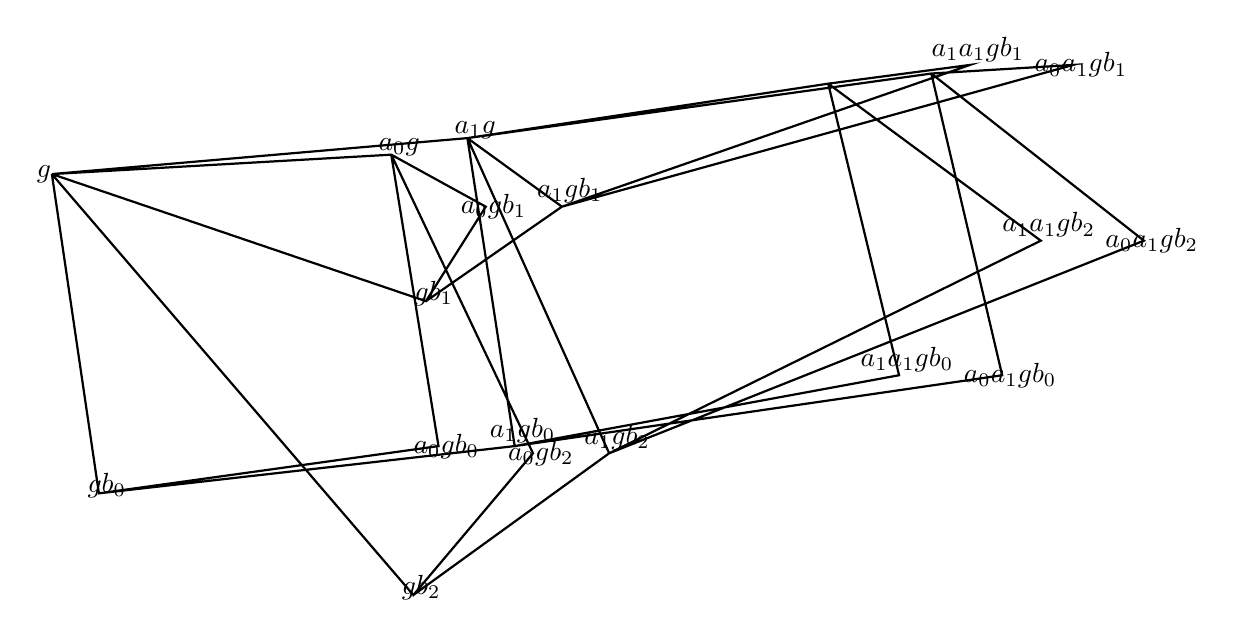
\begin{tikzpicture}
            \draw[thick](0,0)(0, 0) -- (0.5972884314778987,-4.054719970768599) -- (4.910243890273058,-3.454719970768599) -- (4.310243890273059,0.24629678118595488) -- (0, 0)
(0, 0) -- (4.750695261161508,-1.614084329865875) -- (5.510243890273059,-0.41408432986587496) -- (4.310243890273059,0.24629678118595488) -- (0, 0)
(0, 0) -- (4.5909091801856725,-5.345949444351121) -- (6.1102438902730585,-3.5459494443511215) -- (4.310243890273059,0.24629678118595488) -- (0, 0)
(0, 0) -- (0.5972884314778987,-4.054719970768599) -- (5.877516528478765,-3.454719970768599) -- (5.277516528478765,0.45672576464191705) -- (0, 0)
(0, 0) -- (4.750695261161508,-1.614084329865875) -- (6.477516528478765,-0.41408432986587496) -- (5.277516528478765,0.45672576464191705) -- (0, 0)
(0, 0) -- (4.5909091801856725,-5.345949444351121) -- (7.077516528478765,-3.5459494443511215) -- (5.277516528478765,0.45672576464191705) -- (0, 0)
(5.277516528478765, 0.45672576464191705) -- (5.877516528478765,-3.454719970768599) -- (12.068800808503516,-2.5547199707685992) -- (11.168800808503516,1.2768332072142317) -- (5.277516528478765, 0.45672576464191705)
(5.277516528478765, 0.45672576464191705) -- (6.477516528478765,-0.41408432986587496) -- (12.968800808503516,1.385915670134125) -- (11.168800808503516,1.2768332072142317) -- (5.277516528478765, 0.45672576464191705)
(5.277516528478765, 0.45672576464191705) -- (7.077516528478765,-3.5459494443511215) -- (13.868800808503515,-0.8459494443511213) -- (11.168800808503516,1.2768332072142317) -- (5.277516528478765, 0.45672576464191705)
(5.277516528478765, 0.45672576464191705) -- (5.877516528478765,-3.454719970768599) -- (10.759201524682512,-2.5547199707685992) -- (9.859201524682511,1.148134133503106) -- (5.277516528478765, 0.45672576464191705)
(5.277516528478765, 0.45672576464191705) -- (6.477516528478765,-0.41408432986587496) -- (11.659201524682512,1.385915670134125) -- (9.859201524682511,1.148134133503106) -- (5.277516528478765, 0.45672576464191705)
(5.277516528478765, 0.45672576464191705) -- (7.077516528478765,-3.5459494443511215) -- (12.55920152468251,-0.8459494443511213) -- (9.859201524682511,1.148134133503106) -- (5.277516528478765, 0.45672576464191705)
;
\node at (5.010243890273058,-3.454719970768599) {$ a_{ 0  } gb_{ 0 } $};
\node at (5.6102438902730585,-0.41408432986587496) {$ a_{ 0  } gb_{ 1 } $};
\node at (6.210243890273058,-3.5459494443511215) {$ a_{ 0  } gb_{ 2 } $};
\node at (5.977516528478764,-3.254719970768599) {$ a_{ 1  } gb_{ 0 } $};
\node at (6.577516528478765,-0.21408432986587494) {$ a_{ 1  } gb_{ 1 } $};
\node at (7.1775165284787645,-3.3459494443511213) {$ a_{ 1  } gb_{ 2 } $};
\node at (12.168800808503516,-2.5547199707685992) {$ a_{ 0  } a_{ 1 }gb_{ 0 } $};
\node at (13.068800808503516,1.385915670134125) {$ a_{ 0  } a_{ 1 }gb_{ 1 } $};
\node at (13.968800808503515,-0.8459494443511213) {$ a_{ 0  } a_{ 1 }gb_{ 2 } $};
\node at (10.859201524682511,-2.354719970768599) {$ a_{ 1  } a_{ 1 }gb_{ 0 } $};
\node at (11.759201524682512,1.585915670134125) {$ a_{ 1  } a_{ 1 }gb_{ 1 } $};
\node at (12.65920152468251,-0.6459494443511213) {$ a_{ 1  } a_{ 1 }gb_{ 2 } $};
\node at (-0.1,0) {$ g $};
\node at (4.410243890273058,0.34629678118595486) {$ a_{ 0 }g $};
\node at (5.377516528478765,0.556725764641917) {$ a_{ 1 }g $};
\node at (0.6972884314778987,-3.954719970768599) {$ gb_{ 0 } $};
\node at (4.8506952611615075,-1.5140843298658748) {$ gb_{ 1 } $};
\node at (4.690909180185672,-5.245949444351122) {$ gb_{ 2 } $};

            \end{tikzpicture}
            \end{center}
            \caption{Square of the complex, with edges $(g,ag), (agb, gb) \in E_A,
            (g,gb), (agb, ag) \in E_B.$ \label{fig:square}
            }
            \end{figure}
 \begin{figure}[H]
            %\label{fig:square}
            \begin{center}
            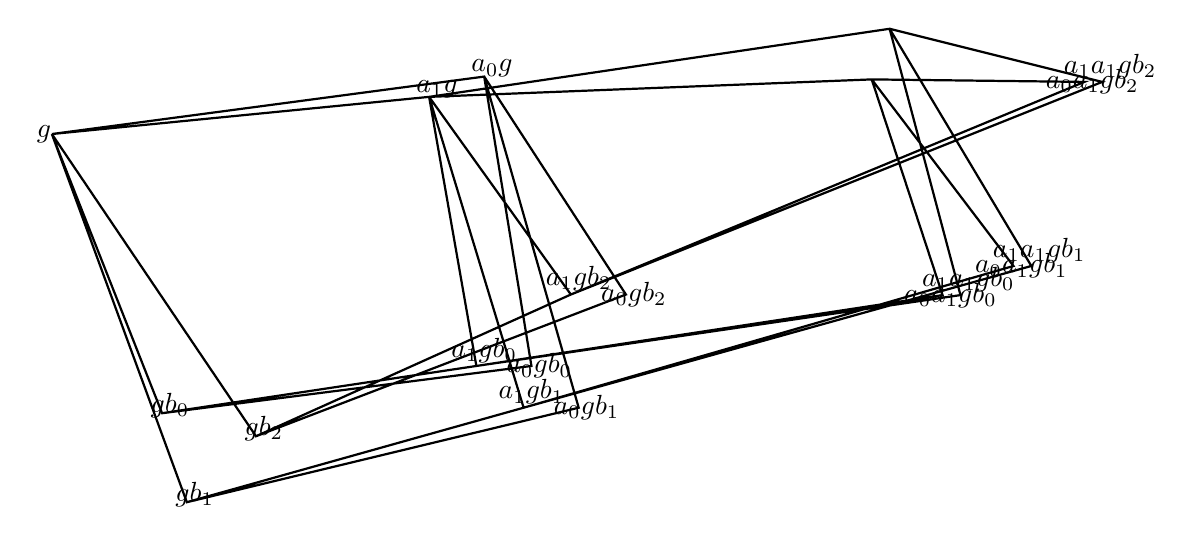
\begin{tikzpicture}
            \draw[thick](0,0)(0, 0) -- (1.3995290181074656,-3.545562707308258) -- (6.090408575862219,-2.945562707308258) -- (5.49040857586222,0.7295978796330752) -- (0, 0)
(0, 0) -- (1.714219417756893,-4.675739131446404) -- (6.69040857586222,-3.475739131446404) -- (5.49040857586222,0.7295978796330752) -- (0, 0)
(0, 0) -- (2.5921510904861607,-3.838243098410442) -- (7.2904085758622195,-2.038243098410442) -- (5.49040857586222,0.7295978796330752) -- (0, 0)
(0, 0) -- (1.3995290181074656,-3.545562707308258) -- (5.391093476839896,-2.945562707308258) -- (4.7910934768398965,0.4718812454878211) -- (0, 0)
(0, 0) -- (1.714219417756893,-4.675739131446404) -- (5.991093476839897,-3.475739131446404) -- (4.7910934768398965,0.4718812454878211) -- (0, 0)
(0, 0) -- (2.5921510904861607,-3.838243098410442) -- (6.591093476839896,-2.038243098410442) -- (4.7910934768398965,0.4718812454878211) -- (0, 0)
(4.7910934768398965, 0.4718812454878211) -- (5.391093476839896,-2.945562707308258) -- (11.311906142944038,-2.045562707308258) -- (10.411906142944037,0.6936532360650072) -- (4.7910934768398965, 0.4718812454878211)
(4.7910934768398965, 0.4718812454878211) -- (5.991093476839897,-3.475739131446404) -- (12.211906142944038,-1.6757391314464039) -- (10.411906142944037,0.6936532360650072) -- (4.7910934768398965, 0.4718812454878211)
(4.7910934768398965, 0.4718812454878211) -- (6.591093476839896,-2.038243098410442) -- (13.111906142944036,0.6617569015895581) -- (10.411906142944037,0.6936532360650072) -- (4.7910934768398965, 0.4718812454878211)
(4.7910934768398965, 0.4718812454878211) -- (5.391093476839896,-2.945562707308258) -- (11.539249904176186,-2.045562707308258) -- (10.639249904176186,1.336631421660789) -- (4.7910934768398965, 0.4718812454878211)
(4.7910934768398965, 0.4718812454878211) -- (5.991093476839897,-3.475739131446404) -- (12.439249904176187,-1.6757391314464039) -- (10.639249904176186,1.336631421660789) -- (4.7910934768398965, 0.4718812454878211)
(4.7910934768398965, 0.4718812454878211) -- (6.591093476839896,-2.038243098410442) -- (13.339249904176185,0.6617569015895581) -- (10.639249904176186,1.336631421660789) -- (4.7910934768398965, 0.4718812454878211)
;
\node at (6.190408575862219,-2.945562707308258) {$ a_{ 0  } gb_{ 0 } $};
\node at (6.7904085758622195,-3.475739131446404) {$ a_{ 0  } gb_{ 1 } $};
\node at (7.390408575862219,-2.038243098410442) {$ a_{ 0  } gb_{ 2 } $};
\node at (5.491093476839896,-2.745562707308258) {$ a_{ 1  } gb_{ 0 } $};
\node at (6.091093476839896,-3.2757391314464037) {$ a_{ 1  } gb_{ 1 } $};
\node at (6.691093476839896,-1.838243098410442) {$ a_{ 1  } gb_{ 2 } $};
\node at (11.411906142944037,-2.045562707308258) {$ a_{ 0  } a_{ 1 }gb_{ 0 } $};
\node at (12.311906142944038,-1.6757391314464039) {$ a_{ 0  } a_{ 1 }gb_{ 1 } $};
\node at (13.211906142944036,0.6617569015895581) {$ a_{ 0  } a_{ 1 }gb_{ 2 } $};
\node at (11.639249904176186,-1.845562707308258) {$ a_{ 1  } a_{ 1 }gb_{ 0 } $};
\node at (12.539249904176186,-1.475739131446404) {$ a_{ 1  } a_{ 1 }gb_{ 1 } $};
\node at (13.439249904176185,0.8617569015895581) {$ a_{ 1  } a_{ 1 }gb_{ 2 } $};
\node at (-0.1,0) {$ g $};
\node at (5.590408575862219,0.8295978796330752) {$ a_{ 0 }g $};
\node at (4.891093476839896,0.5718812454878212) {$ a_{ 1 }g $};
\node at (1.4995290181074656,-3.445562707308258) {$ gb_{ 0 } $};
\node at (1.814219417756893,-4.575739131446404) {$ gb_{ 1 } $};
\node at (2.6921510904861607,-3.738243098410442) {$ gb_{ 2 } $};

            \end{tikzpicture}
            \end{center}
            \caption{Square of the complex, with edges $(g,ag), (agb, gb) \in E_A,
            (g,gb), (agb, ag) \in E_B.$ \label{fig:square}
            }
            \end{figure}
 \begin{figure}[H]
            %\label{fig:square}
            \begin{center}
            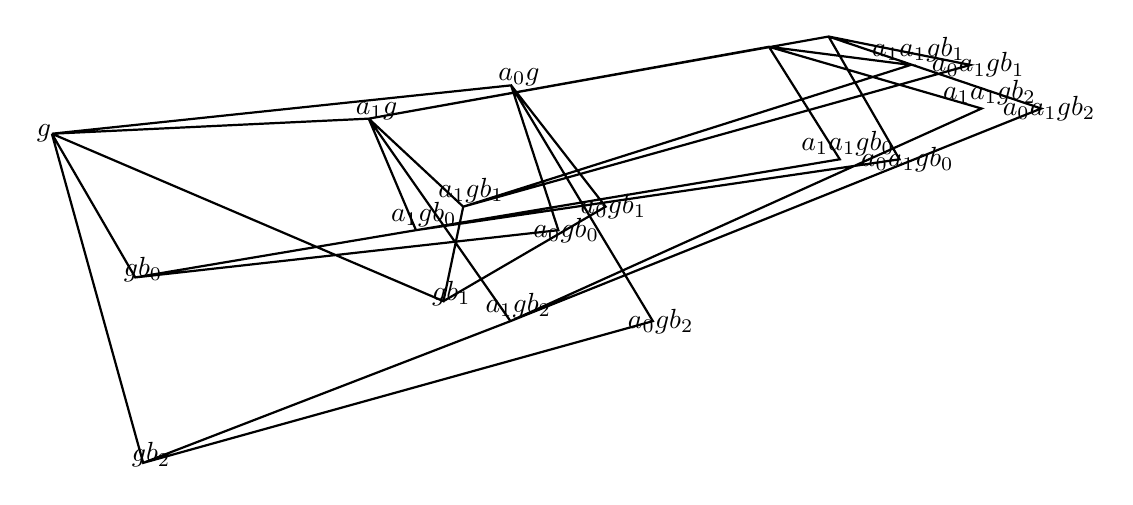
\begin{tikzpicture}
            \draw[thick](0,0)(0, 0) -- (1.0588475787510232,-1.8250345268729005) -- (6.432437233674304,-1.2250345268729004) -- (5.8324372336743044,0.6141384142982355) -- (0, 0)
(0, 0) -- (4.972908770389536,-2.1265578637875784) -- (7.032437233674305,-0.9265578637875784) -- (5.8324372336743044,0.6141384142982355) -- (0, 0)
(0, 0) -- (1.1597708639752835,-4.180022136295601) -- (7.632437233674304,-2.380022136295601) -- (5.8324372336743044,0.6141384142982355) -- (0, 0)
(0, 0) -- (1.0588475787510232,-1.8250345268729005) -- (4.624200011330272,-1.2250345268729004) -- (4.024200011330272,0.19141328616979378) -- (0, 0)
(0, 0) -- (4.972908770389536,-2.1265578637875784) -- (5.2242000113302725,-0.9265578637875784) -- (4.024200011330272,0.19141328616979378) -- (0, 0)
(0, 0) -- (1.1597708639752835,-4.180022136295601) -- (5.824200011330272,-2.380022136295601) -- (4.024200011330272,0.19141328616979378) -- (0, 0)
(4.024200011330272, 0.19141328616979378) -- (4.624200011330272,-1.2250345268729004) -- (10.76420124393105,-0.32503452687290035) -- (9.86420124393105,1.234195420609784) -- (4.024200011330272, 0.19141328616979378)
(4.024200011330272, 0.19141328616979378) -- (5.2242000113302725,-0.9265578637875784) -- (11.66420124393105,0.8734421362124216) -- (9.86420124393105,1.234195420609784) -- (4.024200011330272, 0.19141328616979378)
(4.024200011330272, 0.19141328616979378) -- (5.824200011330272,-2.380022136295601) -- (12.564201243931048,0.3199778637043993) -- (9.86420124393105,1.234195420609784) -- (4.024200011330272, 0.19141328616979378)
(4.024200011330272, 0.19141328616979378) -- (4.624200011330272,-1.2250345268729004) -- (10.006503258324022,-0.32503452687290035) -- (9.106503258324022,1.104207102139646) -- (4.024200011330272, 0.19141328616979378)
(4.024200011330272, 0.19141328616979378) -- (5.2242000113302725,-0.9265578637875784) -- (10.906503258324022,0.8734421362124216) -- (9.106503258324022,1.104207102139646) -- (4.024200011330272, 0.19141328616979378)
(4.024200011330272, 0.19141328616979378) -- (5.824200011330272,-2.380022136295601) -- (11.806503258324021,0.3199778637043993) -- (9.106503258324022,1.104207102139646) -- (4.024200011330272, 0.19141328616979378)
;
\node at (6.532437233674304,-1.2250345268729004) {$ a_{ 0  } gb_{ 0 } $};
\node at (7.132437233674304,-0.9265578637875784) {$ a_{ 0  } gb_{ 1 } $};
\node at (7.732437233674304,-2.380022136295601) {$ a_{ 0  } gb_{ 2 } $};
\node at (4.724200011330272,-1.0250345268729004) {$ a_{ 1  } gb_{ 0 } $};
\node at (5.324200011330272,-0.7265578637875785) {$ a_{ 1  } gb_{ 1 } $};
\node at (5.924200011330272,-2.1800221362956007) {$ a_{ 1  } gb_{ 2 } $};
\node at (10.86420124393105,-0.32503452687290035) {$ a_{ 0  } a_{ 1 }gb_{ 0 } $};
\node at (11.76420124393105,0.8734421362124216) {$ a_{ 0  } a_{ 1 }gb_{ 1 } $};
\node at (12.664201243931048,0.3199778637043993) {$ a_{ 0  } a_{ 1 }gb_{ 2 } $};
\node at (10.106503258324022,-0.12503452687290034) {$ a_{ 1  } a_{ 1 }gb_{ 0 } $};
\node at (11.006503258324022,1.0734421362124216) {$ a_{ 1  } a_{ 1 }gb_{ 1 } $};
\node at (11.90650325832402,0.5199778637043992) {$ a_{ 1  } a_{ 1 }gb_{ 2 } $};
\node at (-0.1,0) {$ g $};
\node at (5.932437233674304,0.7141384142982354) {$ a_{ 0 }g $};
\node at (4.124200011330272,0.2914132861697938) {$ a_{ 1 }g $};
\node at (1.1588475787510233,-1.7250345268729004) {$ gb_{ 0 } $};
\node at (5.072908770389535,-2.0265578637875783) {$ gb_{ 1 } $};
\node at (1.2597708639752836,-4.080022136295601) {$ gb_{ 2 } $};

            \end{tikzpicture}
            \end{center}
            \caption{Square of the complex, with edges $(g,ag), (agb, gb) \in E_A,
            (g,gb), (agb, ag) \in E_B.$ \label{fig:square}
            }
            \end{figure}
 \begin{figure}[H]
            %\label{fig:square}
            \begin{center}
            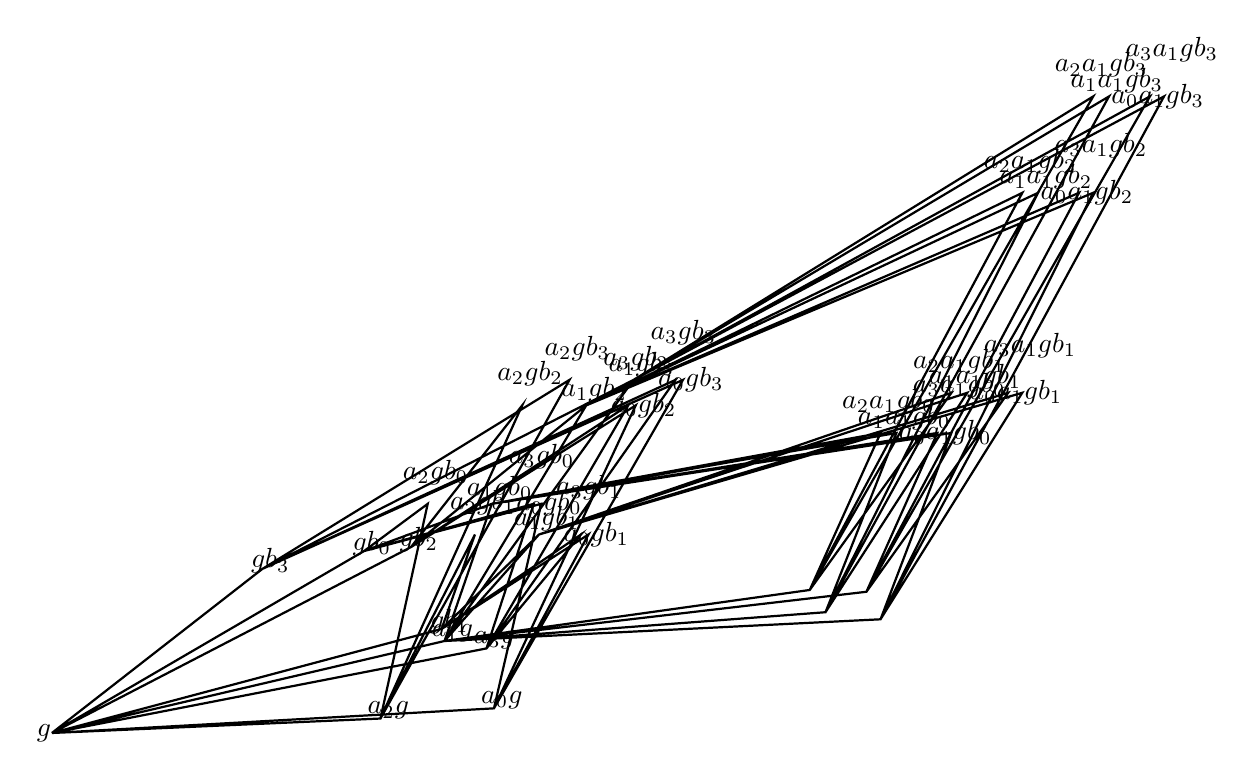
\begin{tikzpicture}
            \draw[thick](0,0)(0, 0) -- (3.964212557659967,2.3101181861008913) -- (6.214534600028168,2.9101181861008913) -- (5.614534600028168,0.3128467638804855) -- (0, 0)
(0, 0) -- (4.948865754034145,1.3205671838883157) -- (6.814534600028169,2.520567183888316) -- (5.614534600028168,0.3128467638804855) -- (0, 0)
(0, 0) -- (4.5599372199385595,2.360342732789619) -- (7.414534600028168,4.160342732789619) -- (5.614534600028168,0.3128467638804855) -- (0, 0)
(0, 0) -- (2.673922771152317,2.084065753099584) -- (8.014534600028169,4.484065753099584) -- (5.614534600028168,0.3128467638804855) -- (0, 0)
(0, 0) -- (3.964212557659967,2.3101181861008913) -- (5.586834333410329,2.9101181861008913) -- (4.98683433341033,1.1682153983161898) -- (0, 0)
(0, 0) -- (4.948865754034145,1.3205671838883157) -- (6.18683433341033,2.520567183888316) -- (4.98683433341033,1.1682153983161898) -- (0, 0)
(0, 0) -- (4.5599372199385595,2.360342732789619) -- (6.786834333410329,4.160342732789619) -- (4.98683433341033,1.1682153983161898) -- (0, 0)
(0, 0) -- (2.673922771152317,2.084065753099584) -- (7.386834333410329,4.484065753099584) -- (4.98683433341033,1.1682153983161898) -- (0, 0)
(0, 0) -- (3.964212557659967,2.3101181861008913) -- (4.773156464837455,2.9101181861008913) -- (4.173156464837455,0.1836075358456699) -- (0, 0)
(0, 0) -- (4.948865754034145,1.3205671838883157) -- (5.3731564648374555,2.520567183888316) -- (4.173156464837455,0.1836075358456699) -- (0, 0)
(0, 0) -- (4.5599372199385595,2.360342732789619) -- (5.973156464837455,4.160342732789619) -- (4.173156464837455,0.1836075358456699) -- (0, 0)
(0, 0) -- (2.673922771152317,2.084065753099584) -- (6.573156464837455,4.484065753099584) -- (4.173156464837455,0.1836075358456699) -- (0, 0)
(0, 0) -- (3.964212557659967,2.3101181861008913) -- (6.119542001490748,2.9101181861008913) -- (5.519542001490748,1.0738094009949843) -- (0, 0)
(0, 0) -- (4.948865754034145,1.3205671838883157) -- (6.7195420014907485,2.520567183888316) -- (5.519542001490748,1.0738094009949843) -- (0, 0)
(0, 0) -- (4.5599372199385595,2.360342732789619) -- (7.319542001490748,4.160342732789619) -- (5.519542001490748,1.0738094009949843) -- (0, 0)
(0, 0) -- (2.673922771152317,2.084065753099584) -- (7.919542001490749,4.484065753099584) -- (5.519542001490748,1.0738094009949843) -- (0, 0)
(4.98683433341033, 1.1682153983161898) -- (5.586834333410329,2.9101181861008913) -- (11.24491596605919,3.8101181861008913) -- (10.34491596605919,1.7933329268038638) -- (4.98683433341033, 1.1682153983161898)
(4.98683433341033, 1.1682153983161898) -- (6.18683433341033,2.520567183888316) -- (12.144915966059191,4.320567183888316) -- (10.34491596605919,1.7933329268038638) -- (4.98683433341033, 1.1682153983161898)
(4.98683433341033, 1.1682153983161898) -- (6.786834333410329,4.160342732789619) -- (13.04491596605919,6.860342732789619) -- (10.34491596605919,1.7933329268038638) -- (4.98683433341033, 1.1682153983161898)
(4.98683433341033, 1.1682153983161898) -- (7.386834333410329,4.484065753099584) -- (13.94491596605919,8.084065753099583) -- (10.34491596605919,1.7933329268038638) -- (4.98683433341033, 1.1682153983161898)
(4.98683433341033, 1.1682153983161898) -- (5.586834333410329,2.9101181861008913) -- (10.725138667171416,3.8101181861008913) -- (9.825138667171416,1.5337235857651612) -- (4.98683433341033, 1.1682153983161898)
(4.98683433341033, 1.1682153983161898) -- (6.18683433341033,2.520567183888316) -- (11.625138667171417,4.320567183888316) -- (9.825138667171416,1.5337235857651612) -- (4.98683433341033, 1.1682153983161898)
(4.98683433341033, 1.1682153983161898) -- (6.786834333410329,4.160342732789619) -- (12.525138667171415,6.860342732789619) -- (9.825138667171416,1.5337235857651612) -- (4.98683433341033, 1.1682153983161898)
(4.98683433341033, 1.1682153983161898) -- (7.386834333410329,4.484065753099584) -- (13.425138667171415,8.084065753099583) -- (9.825138667171416,1.5337235857651612) -- (4.98683433341033, 1.1682153983161898)
(4.98683433341033, 1.1682153983161898) -- (5.586834333410329,2.9101181861008913) -- (10.524769124320079,3.8101181861008913) -- (9.624769124320078,1.8161042671218843) -- (4.98683433341033, 1.1682153983161898)
(4.98683433341033, 1.1682153983161898) -- (6.18683433341033,2.520567183888316) -- (11.424769124320079,4.320567183888316) -- (9.624769124320078,1.8161042671218843) -- (4.98683433341033, 1.1682153983161898)
(4.98683433341033, 1.1682153983161898) -- (6.786834333410329,4.160342732789619) -- (12.324769124320078,6.860342732789619) -- (9.624769124320078,1.8161042671218843) -- (4.98683433341033, 1.1682153983161898)
(4.98683433341033, 1.1682153983161898) -- (7.386834333410329,4.484065753099584) -- (13.224769124320078,8.084065753099583) -- (9.624769124320078,1.8161042671218843) -- (4.98683433341033, 1.1682153983161898)
(4.98683433341033, 1.1682153983161898) -- (5.586834333410329,2.9101181861008913) -- (11.423892040676632,3.8101181861008913) -- (10.523892040676632,1.4438474130007422) -- (4.98683433341033, 1.1682153983161898)
(4.98683433341033, 1.1682153983161898) -- (6.18683433341033,2.520567183888316) -- (12.323892040676633,4.320567183888316) -- (10.523892040676632,1.4438474130007422) -- (4.98683433341033, 1.1682153983161898)
(4.98683433341033, 1.1682153983161898) -- (6.786834333410329,4.160342732789619) -- (13.223892040676631,6.860342732789619) -- (10.523892040676632,1.4438474130007422) -- (4.98683433341033, 1.1682153983161898)
(4.98683433341033, 1.1682153983161898) -- (7.386834333410329,4.484065753099584) -- (14.123892040676632,8.084065753099583) -- (10.523892040676632,1.4438474130007422) -- (4.98683433341033, 1.1682153983161898)
;
\node at (6.314534600028168,2.9101181861008913) {$ a_{ 0  } gb_{ 0 } $};
\node at (6.914534600028168,2.520567183888316) {$ a_{ 0  } gb_{ 1 } $};
\node at (7.514534600028168,4.160342732789619) {$ a_{ 0  } gb_{ 2 } $};
\node at (8.114534600028168,4.484065753099584) {$ a_{ 0  } gb_{ 3 } $};
\node at (5.686834333410329,3.1101181861008915) {$ a_{ 1  } gb_{ 0 } $};
\node at (6.286834333410329,2.720567183888316) {$ a_{ 1  } gb_{ 1 } $};
\node at (6.886834333410329,4.360342732789619) {$ a_{ 1  } gb_{ 2 } $};
\node at (7.486834333410329,4.684065753099584) {$ a_{ 1  } gb_{ 3 } $};
\node at (4.873156464837455,3.3101181861008913) {$ a_{ 2  } gb_{ 0 } $};
\node at (5.473156464837455,2.920567183888316) {$ a_{ 2  } gb_{ 1 } $};
\node at (6.073156464837455,4.5603427327896195) {$ a_{ 2  } gb_{ 2 } $};
\node at (6.673156464837454,4.884065753099584) {$ a_{ 2  } gb_{ 3 } $};
\node at (6.219542001490748,3.5101181861008914) {$ a_{ 3  } gb_{ 0 } $};
\node at (6.819542001490748,3.120567183888316) {$ a_{ 3  } gb_{ 1 } $};
\node at (7.419542001490748,4.760342732789619) {$ a_{ 3  } gb_{ 2 } $};
\node at (8.019542001490748,5.084065753099583) {$ a_{ 3  } gb_{ 3 } $};
\node at (11.34491596605919,3.8101181861008913) {$ a_{ 0  } a_{ 1 }gb_{ 0 } $};
\node at (12.24491596605919,4.320567183888316) {$ a_{ 0  } a_{ 1 }gb_{ 1 } $};
\node at (13.14491596605919,6.860342732789619) {$ a_{ 0  } a_{ 1 }gb_{ 2 } $};
\node at (14.04491596605919,8.084065753099583) {$ a_{ 0  } a_{ 1 }gb_{ 3 } $};
\node at (10.825138667171416,4.010118186100891) {$ a_{ 1  } a_{ 1 }gb_{ 0 } $};
\node at (11.725138667171416,4.520567183888316) {$ a_{ 1  } a_{ 1 }gb_{ 1 } $};
\node at (12.625138667171415,7.0603427327896195) {$ a_{ 1  } a_{ 1 }gb_{ 2 } $};
\node at (13.525138667171415,8.284065753099583) {$ a_{ 1  } a_{ 1 }gb_{ 3 } $};
\node at (10.624769124320078,4.210118186100892) {$ a_{ 2  } a_{ 1 }gb_{ 0 } $};
\node at (11.524769124320079,4.720567183888316) {$ a_{ 2  } a_{ 1 }gb_{ 1 } $};
\node at (12.424769124320077,7.26034273278962) {$ a_{ 2  } a_{ 1 }gb_{ 2 } $};
\node at (13.324769124320078,8.484065753099584) {$ a_{ 2  } a_{ 1 }gb_{ 3 } $};
\node at (11.523892040676632,4.410118186100892) {$ a_{ 3  } a_{ 1 }gb_{ 0 } $};
\node at (12.423892040676632,4.920567183888316) {$ a_{ 3  } a_{ 1 }gb_{ 1 } $};
\node at (13.32389204067663,7.46034273278962) {$ a_{ 3  } a_{ 1 }gb_{ 2 } $};
\node at (14.223892040676631,8.684065753099583) {$ a_{ 3  } a_{ 1 }gb_{ 3 } $};
\node at (-0.1,0) {$ g $};
\node at (5.714534600028168,0.41284676388048547) {$ a_{ 0 }g $};
\node at (5.086834333410329,1.26821539831619) {$ a_{ 1 }g $};
\node at (4.273156464837455,0.2836075358456699) {$ a_{ 2 }g $};
\node at (5.619542001490748,1.1738094009949844) {$ a_{ 3 }g $};
\node at (4.064212557659967,2.4101181861008913) {$ gb_{ 0 } $};
\node at (5.048865754034145,1.4205671838883158) {$ gb_{ 1 } $};
\node at (4.659937219938559,2.460342732789619) {$ gb_{ 2 } $};
\node at (2.773922771152317,2.184065753099584) {$ gb_{ 3 } $};

            \end{tikzpicture}
            \end{center}
            \caption{Square of the complex, with edges $(g,ag), (agb, gb) \in E_A,
            (g,gb), (agb, ag) \in E_B.$ \label{fig:square}
            }
            \end{figure}
 
%\end{multicols*}
  % \printbibliography 
\end{document}

 